%==============================================================================
% Figure: Framework Comparison Table (Visual)
% Purpose: Side-by-side comparison of Aether, Genesis, and Pais frameworks
% Chapter: Ch17 - Framework Comparison and Reconciliation
% Type: Comparative table / Feature matrix
%==============================================================================

\begin{figure}[htbp]
  \centering
  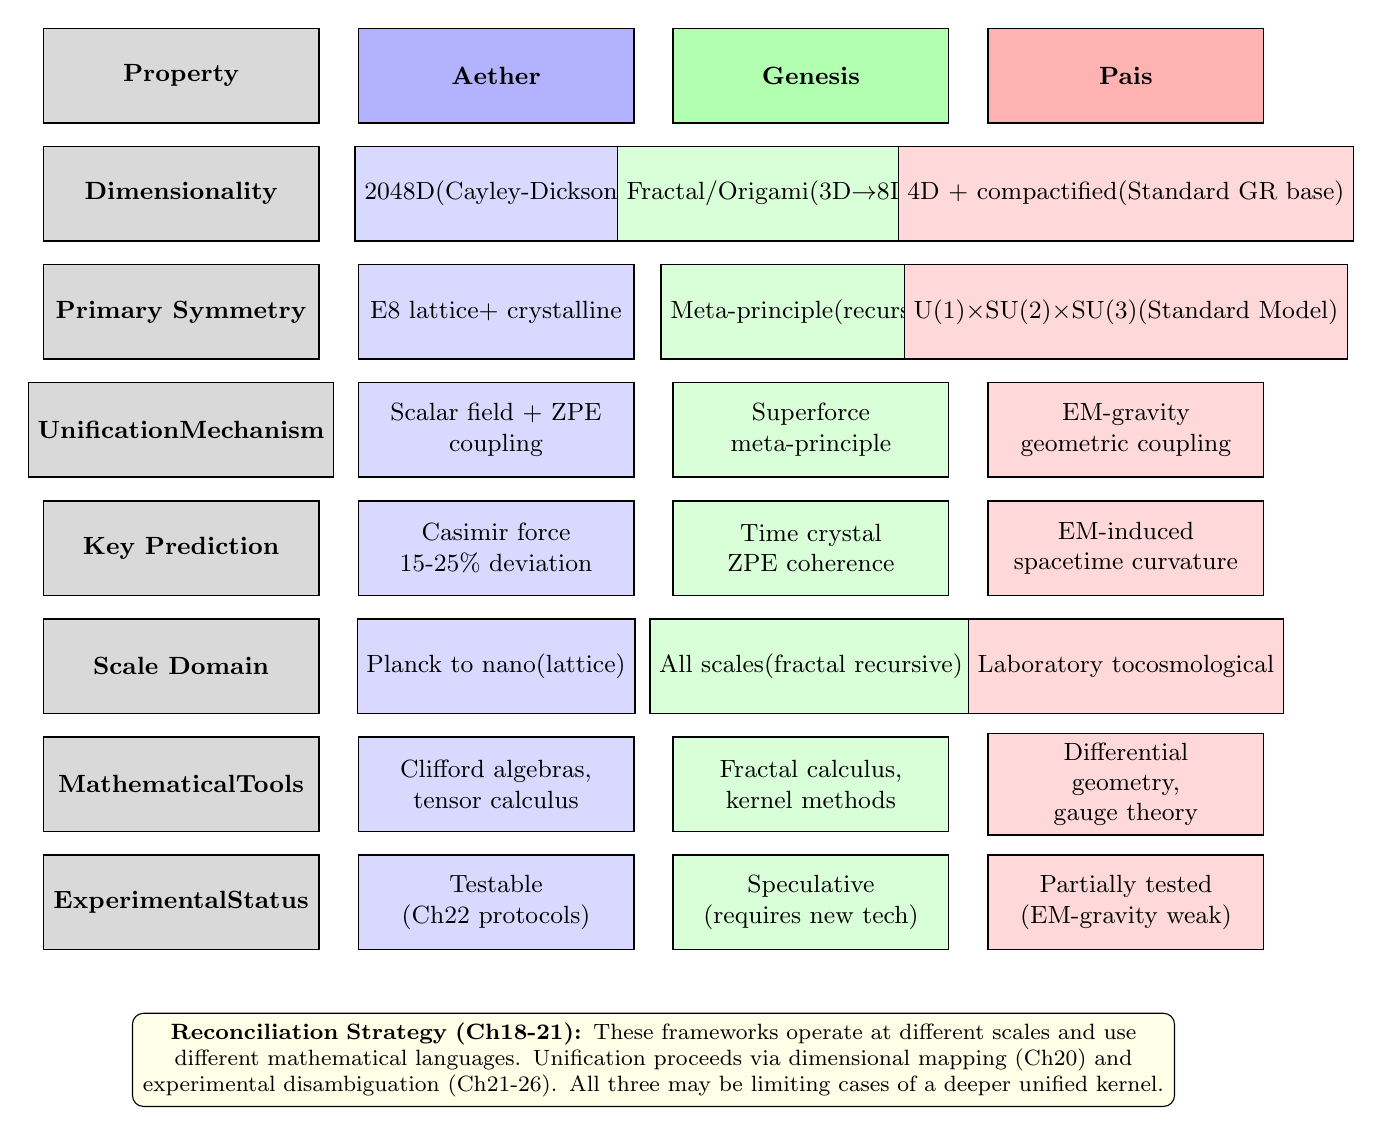
\begin{tikzpicture}[
    cell/.style={
      rectangle,
      draw=black,
      line width=0.5pt,
      minimum width=3.5cm,
      minimum height=1.2cm,
      text centered,
      font=\small
    },
    header/.style={
      cell,
      fill=gray!30,
      font=\small\bfseries
    },
    aether/.style={
      cell,
      fill=blue!15
    },
    genesis/.style={
      cell,
      fill=green!15
    },
    pais/.style={
      cell,
      fill=red!15
    }
  ]

    % Column headers
    \node[header] at (0,0) {Property};
    \node[header, fill=blue!30] at (4,0) {Aether};
    \node[header, fill=green!30] at (8,0) {Genesis};
    \node[header, fill=red!30] at (12,0) {Pais};

    % Row 1: Dimensionality
    \node[header, minimum width=3.5cm] at (0,-1.5) {Dimensionality};
    \node[aether] at (4,-1.5) {2048D\\(Cayley-Dickson)};
    \node[genesis] at (8,-1.5) {Fractal/Origami\\(3D$\to$8D folded)};
    \node[pais] at (12,-1.5) {4D + compactified\\(Standard GR base)};

    % Row 2: Primary Symmetry
    \node[header] at (0,-3) {Primary Symmetry};
    \node[aether] at (4,-3) {E8 lattice\\+ crystalline};
    \node[genesis] at (8,-3) {Meta-principle\\(recursive)};
    \node[pais] at (12,-3) {U(1)$\times$SU(2)$\times$SU(3)\\(Standard Model)};

    % Row 3: Unification Mechanism
    \node[header] at (0,-4.5) {Unification\\Mechanism};
    \node[aether, text width=3cm, align=center] at (4,-4.5) {Scalar field + ZPE\\coupling};
    \node[genesis, text width=3cm, align=center] at (8,-4.5) {Superforce\\meta-principle};
    \node[pais, text width=3cm, align=center] at (12,-4.5) {EM-gravity\\geometric coupling};

    % Row 4: Key Prediction
    \node[header] at (0,-6) {Key Prediction};
    \node[aether, text width=3cm, align=center] at (4,-6) {Casimir force\\15-25\% deviation};
    \node[genesis, text width=3cm, align=center] at (8,-6) {Time crystal\\ZPE coherence};
    \node[pais, text width=3cm, align=center] at (12,-6) {EM-induced\\spacetime curvature};

    % Row 5: Scale Domain
    \node[header] at (0,-7.5) {Scale Domain};
    \node[aether] at (4,-7.5) {Planck to nano\\(lattice)};
    \node[genesis] at (8,-7.5) {All scales\\(fractal recursive)};
    \node[pais] at (12,-7.5) {Laboratory to\\cosmological};

    % Row 6: Mathematical Tools
    \node[header] at (0,-9) {Mathematical\\Tools};
    \node[aether, text width=3cm, align=center] at (4,-9) {Clifford algebras,\\tensor calculus};
    \node[genesis, text width=3cm, align=center] at (8,-9) {Fractal calculus,\\kernel methods};
    \node[pais, text width=3cm, align=center] at (12,-9) {Differential geometry,\\gauge theory};

    % Row 7: Experimental Status
    \node[header] at (0,-10.5) {Experimental\\Status};
    \node[aether, text width=3cm, align=center] at (4,-10.5) {Testable\\(Ch22 protocols)};
    \node[genesis, text width=3cm, align=center] at (8,-10.5) {Speculative\\(requires new tech)};
    \node[pais, text width=3cm, align=center] at (12,-10.5) {Partially tested\\(EM-gravity weak)};

    % Bottom note
    \node[
      draw,
      rounded corners,
      fill=yellow!10,
      text width=13cm,
      align=center,
      font=\footnotesize
    ] at (6,-12.5) {
      \textbf{Reconciliation Strategy (Ch18-21):} These frameworks operate at different scales
      and use different mathematical languages. Unification proceeds via dimensional mapping
      (Ch20) and experimental disambiguation (Ch21-26). All three may be limiting cases of
      a deeper unified kernel.
    };

  \end{tikzpicture}

  \caption{Comparative matrix of the three major theoretical frameworks synthesized in this monograph. The Aether framework emphasizes crystalline lattice structure at microscopic scales; Genesis employs fractal/recursive meta-principles across all scales; Pais focuses on electromagnetic-gravitational coupling within standard geometric frameworks. Color coding: blue (Aether), green (Genesis), red (Pais). These frameworks are not mutually exclusive but rather complementary descriptions that may emerge from a unified kernel structure (Part III).}
  \label{fig:framework-comparison}
\end{figure}
